\section{Projektbeschreibung}

Das Projekt AudioNEXT analysiert ein per 3,5 mm Klinke eingehendes Audiosignal mit einem Pmod I2S2.
Die aktuelle, durchschnittliche Lautstärke wird über einen Pmod VGA mit 640x480@60Hz ausgegeben.
Die Ausgabe erfolgt dabei im Textformat.

\subsection{Blockdiagramm}

\begin{figure}[h!]
    \centering
    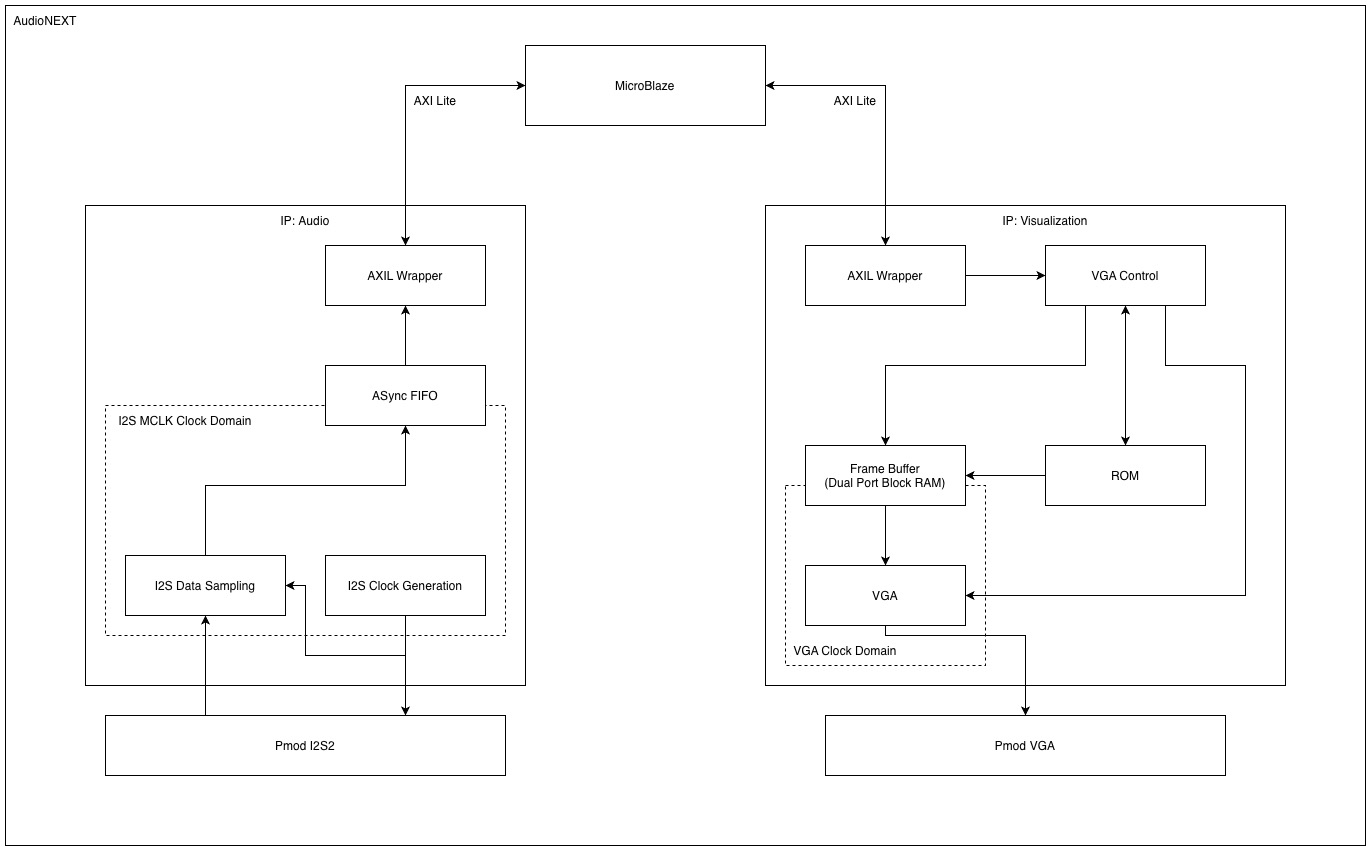
\includegraphics[width=1\textwidth]{files/AudioNEXT_DieAudiophilen}
    \label{fig:block_diagram}
\end{figure}

\subsubsection{IP: Audio}

Der Audio-IP empfängt das Audio Signal vom Pmod I2S2 via I2S im Master Modus mit einer Samplingrate von 96 kHz pro Kanal.
Dazu werden die notwendigen Taktsignale für MCLK, LRCK und SCLK erzeugt.
Das I2S Signal des Pmods wird empfangen und in einen asynchronen FIFO per AXI Stream geladen.
Dort werden die Werte gepuffert und wechseln zudem in die Taktdomäne der AXI Lite Schnittstelle.
Die Daten werden über AXI Lite an den Microblaze übergeben.
Dazu werden Interrupts ausgelöst, wenn ein neuer Wert vorhanden ist.

\subsubsection{MicroBlaze}

Der MicroBlaze berechnet von den Daten des Audio-IPs die Lautstärke und gibt das Ergebnis zur Visualisierung an den Visualization-IP.
Dazu liest er die Daten in Bursts vom Audio-IP über die AXI Lite Schnittstelle.
Um die Lautstärke des Audiosignals zu berechnen werden die beiden Audiokanäle zusammengefasst und der quadratische Mittelwert über mehrere Signalwerte berechnet.

\subsubsection{IP: Visualization}

Der Visualization-IP erhält vom MicroBlaze über AXI Lite die Lautstärke in Prozent als Festkommazahl im 7.2 Format.
Diese wird als Text in den Framebuffer geladen.
Zusätzlich wird die Lautstärke als Balken relativ zum Prozentwert ebenfalls in den Framebuffer geladen.
Das VGA Signal wird im Format 640x480@60Hz erzeugt.
Die Pixelclock dazu wird, ebenso wie Steuersignale, die den aktuellen Status des VGA Signals enthalten, erzeugt.
Der Framebuffer wird zwischen zwei Frames aktualisiert, während sich das VGA Signal in der \glqq Blanking Period\grqq \ befindet.